%\documentclass[12pt]{article} %% required

%% style for page

\documentclass[letterpaper,12pt]{article}
\usepackage{epsfig,colortbl}
\usepackage{amssymb}
\textwidth=6.5in
\textheight=9.5in
\topmargin=-0.75in
\oddsidemargin=0.0in
\evensidemargin=0.0in
\thispagestyle{empty} % no page numbers

\usepackage{times}
\usepackage{psfig}

%%%%% Main Body %%%%%
\begin{document} %% required

{\Large \textbf{Homework 3.0}} \hfill {\small \emph{AST 422 Spring 2007}}\\

\centerline{\psfig{file=kaz_rad.ps,width=0.75\textwidth}}

\vspace{0.5cm}
\noindent Dark Gravitational Lensing?
\begin{itemize}
\item[(a)] Assume the radio source with $S_{1.4GHz}=33$ mJy.\\
Optical  $V$ $\geq$25.0 mag (HST), and $K$ $\geq$19.0 mag.\\
Use Longair Ch 2 to estimate the dark lens' \emph{minimum} $z$.\\

\begin{itemize}
\vspace{-0.7cm}
\item From Fig. 2.9 of Longair, you can simply read off the redshifts 
(\emph{z}).
\item[(i)] $V \geq 25.0$ mag\\
Since the graph only goes up to $V = 20$ mag, you have to extend the graph
or find the slope and plug in when $V = 25.0$ mag.\\
From here, I found that $z_V \sim 9$, which is too far.  But the graph
is particuraly for the ``brightest galaxies in rich cluster'' so this
answer might be unreliable.

\item[(ii)] $K \geq 19.0$ mag\\
This can be found from figure directly, and since the graph is particularly 
for radio galaxies there should be no bias or contamination.  
According to the graph, $K$$=$$19.0$ mag gives you $z_K$$\sim$$3.1$.

\item Since what we looking for is the \emph{minimum} $z$, from the above 
reasoning, $z_{lens}$$=$$3.1$.

\end{itemize}

\item[(b)] Lensed arc background galaxy has $V$ = 24.8 mag.\\
Use Longair Ch 18 (Fig. 18.8) to estimate its \emph{maximum} $z$.\\
Hint: Lynman break occures at $\lambda_{L_{\alpha}}=1216 \AA$ at $z=0$.\\

\begin{itemize}
\vspace{-0.7cm}
\item Fig. 18.8 uses the idea of photometric redshift.\\
To be detected with $V$ band, the spectrum of lensed galaxy must 
have the Lynman limit at $\lambda_V$$\lesssim$$6000 \AA$.  At $z$$=$$0$, 
Lyman break lies at $\lambda_{L_{\alpha}}$$=$$1216 \AA$.  Therefore, 
the maximum wavelength of Lyman break for the observed arc galaxy is 
at $\lambda_{L_{\alpha}}\sim6000 \AA$.  Which means\\
$z_{arc}\sim6000/1216-1\sim3.9$.

\end{itemize}
\item[(c)] Use Longair Ch 4.3.4 to estimate the mass inside the 
Einstein Radius of the dark lens.\\
Remember you can use the Ned Wright's Cosmology Calculator:\\
http://www.astro.ucla.edu/~wright/CosmoCalc.html

\begin{itemize}
\vspace{-0.5cm}
\item The equation we need in Longair 4.3.4 is eq 4.35:
\vspace{-0.3cm}
\[ 
\theta_E = 3 \times 10^{-6} \left(\frac{M}{M_{\odot}}\right)^{1/2} \frac{1}{D_{Gpc}^{1/2}} 
\]

\vspace{-0.3cm}
and By Ned Wright's Cosmology Calculator with default values and Flat 
cosmology, angular diameter distances are:  $D_s(z$$=$$3.9)=1475.9$ Mpc and 
$D_d(z$$=$$3.1)=1599.5$ Mpc.  From the definition of $D_{ds}=D_s-D_d$, the 
value of $D_{ds}$ is therefore, $-83.6$ Mpc.\\
Assuming the arc is part of a perfect circle, the measured radius is
is $\theta_E=2.7$ arcsec.\\
Since $D_{Gpc} = \frac{D_s D_d}{D_{ds}}$ in Gpc instead of Mpc, using the
absolute value for $D_{ds}$, the calculated mass within the Einstein ring is:
\[
M = \left( \frac{\theta_E^2 D_{Gpc}}{(3\times10^{_6})^2}\right) M_{\odot} = 2.23\times10^{13} M_\odot
\]

\end{itemize}
\end{itemize}


\end{document} %% required
